% !TEX TS-program = pdflatex
% academicthesis-introduction.tex
% An introduction to the academicthesis class and to its LUISS and
% Politecnico di Milano packages. Compile from this folder with pdfLaTeX
% (twice, for the table of contents and cross-references):
%   pdflatex academicthesis-introduction.tex
% It is a standalone document: it does not need the academicthesis class.
\documentclass[11pt,a4paper]{article}
\newcommand{\doctitleshort}{academicthesis --- Introduction}
% academicthesis-docstyle.tex
% Shared preamble of the academicthesis documentation (introduction and
% user guide). \input it right after \documentclass. Standalone: the
% documentation does not need the academicthesis class itself.
\usepackage[T1]{fontenc}
\usepackage[utf8]{inputenc}
\usepackage{lmodern}
\usepackage[english]{babel}
\usepackage[a4paper, margin=2.6cm, headheight=14pt]{geometry}
\usepackage{microtype}
\usepackage{xcolor}
\usepackage{graphicx}
\usepackage{array}
\usepackage{tabularx}
\usepackage{booktabs}
\usepackage{longtable}
\usepackage{listings}
\usepackage{enumitem}
\usepackage{titlesec}
\usepackage{fancyhdr}
\usepackage{tcolorbox}
\tcbuselibrary{skins, breakable}
\usepackage{tikz}
\usetikzlibrary{positioning, arrows.meta, fit}
\usepackage{url}
\usepackage[colorlinks=true, linkcolor=docaccent, urlcolor=docaccent,
            citecolor=docaccent]{hyperref}

% ---- Colours ---------------------------------------------------------
\definecolor{docaccent}{RGB}{31,73,125}   % neutral blue for headings
\definecolor{luissblue}{RGB}{21,57,108}   % BlueLuiss, as in the package
\definecolor{bluepoli}{cmyk}{0.4,0.1,0,0.4} % bluepoli, as in the package
\definecolor{docgrey}{gray}{0.45}

% ---- Page and paragraphs --------------------------------------------
\setlength{\parindent}{0pt}
\setlength{\parskip}{0.55\baselineskip}
\setlength{\emergencystretch}{3em}
\setlist{nosep, topsep=3pt, leftmargin=1.5em}
\renewcommand{\arraystretch}{1.25}

\titleformat{\section}{\color{docaccent}\normalfont\Large\bfseries}{\thesection}{0.8em}{}
\titleformat{\subsection}{\color{docaccent}\normalfont\large\bfseries}{\thesubsection}{0.8em}{}
\titleformat{\subsubsection}{\normalfont\normalsize\bfseries}{\thesubsubsection}{0.8em}{}
\titlespacing*{\section}{0pt}{2.2ex plus 1ex}{1ex}

\pagestyle{fancy}
\fancyhf{}
\fancyhead[L]{\small\color{docgrey}\doctitleshort}
\fancyhead[R]{\small\color{docgrey}\nouppercase{\leftmark}}
\fancyfoot[C]{\small\thepage}
\renewcommand{\headrulewidth}{0.3pt}
\renewcommand{\sectionmark}[1]{\markboth{\thesection\quad #1}{}}
\fancypagestyle{plain}{\fancyhf{}\renewcommand{\headrulewidth}{0pt}\fancyfoot[C]{\small\thepage}}
\providecommand{\doctitleshort}{academicthesis}

% ---- Names in running text and tables -------------------------------
\newcommand{\cs}[1]{\texttt{\textbackslash#1}}   % a command
\newcommand{\opt}[1]{\texttt{#1}}                 % an option / key / value
\newcommand{\env}[1]{\texttt{#1}}                 % an environment
\newcommand{\pkg}[1]{\textsf{#1}}                 % a package or class
\DeclareUrlCommand{\file}{\urlstyle{tt}}          % a file name (breaks at - . /)
\renewcommand{\UrlBreaks}{\do\-\do\.\do\/}
\newcolumntype{Y}{>{\raggedright\arraybackslash}X}
\newcolumntype{L}[1]{>{\raggedright\arraybackslash}p{#1}}
\newcommand{\req}{\textbf{required}}
\newcommand{\optional}{optional}
\newcommand{\na}{\textcolor{docgrey}{---}}

% ---- Code listings ----------------------------------------------------
\lstset{
  basicstyle=\ttfamily\small,
  keywordstyle=\color{docaccent}\bfseries,
  commentstyle=\color{docgrey}\itshape,
  language=[LaTeX]TeX,
  morekeywords={thesissetup, frontpage, luissthesissetup, polimithesissetup,
    major, dedication, frontmatter, mainmatter, backmatter, addbibresource,
    printbibliography, blankpage},
  frame=single, rulecolor=\color{docaccent!35},
  backgroundcolor=\color{docaccent!4},
  columns=fullflexible, keepspaces=true, upquote=true,
  xleftmargin=4pt, xrightmargin=4pt, aboveskip=8pt, belowskip=8pt,
  literate={à}{{\`a}}1 {è}{{\`e}}1 {é}{{\'e}}1 {ò}{{\`o}}1,
}
\lstdefinestyle{shell}{language={}, keywordstyle={}, commentstyle={}}

% ---- Boxes -----------------------------------------------------------
% \begin{notebox}{Title} ... \end{notebox}
\newtcolorbox{notebox}[2][docaccent]{enhanced, breakable,
  colback=#1!5, colframe=#1!70, boxrule=0.6pt, arc=2pt,
  left=8pt, right=8pt, top=6pt, bottom=6pt,
  fonttitle=\bfseries\small, coltitle=white, title={#2}}

% A framed page preview: \preview[<width>]{<file>}{<caption>}
\newcommand{\preview}[3][0.42\textwidth]{%
  \begin{minipage}[t]{#1}\centering
    {\setlength{\fboxsep}{0pt}\setlength{\fboxrule}{0.5pt}%
     \fcolorbox{docgrey!50}{white}{\includegraphics[width=\dimexpr\linewidth-1pt\relax]{#2}}}\par
    \vspace{4pt}{\small #3}
  \end{minipage}}

\graphicspath{{figures/}}


\hypersetup{pdftitle={academicthesis: an introduction to the LUISS and Politecnico di Milano packages},
            pdfauthor={Luca Salvatore}}

\begin{document}

% ======================================================================
% Title page
% ======================================================================
\hypersetup{pageanchor=false}
\begin{titlepage}
  \thispagestyle{empty}
  \vspace*{3cm}
  {\color{docaccent}\rule{\linewidth}{1.2pt}}\par\vspace{14pt}
  {\fontsize{30}{36}\selectfont\bfseries\color{docaccent} academicthesis\par}
  \vspace{10pt}
  {\LARGE One thesis class, one package per university\par}
  \vspace{6pt}
  {\Large An introduction to the LUISS and Politecnico di Milano packages\par}
  \vspace{14pt}
  {\color{docaccent}\rule{\linewidth}{1.2pt}}\par
  \vspace{2cm}
  \begin{center}
    \preview[0.3\textwidth]{luiss-master-cover}{LUISS}\hspace{1.2cm}%
    \preview[0.3\textwidth]{polimi-classical-cover}{Politecnico di Milano}
  \end{center}
  \vfill
  {\large Luca Salvatore\par}
  {\color{docgrey} Class version 0.2.0 \quad\textbullet\quad October 2026\par}
\end{titlepage}
\hypersetup{pageanchor=true}

{\setlength{\parskip}{0pt}\tableofcontents}
\clearpage

% ======================================================================
\section{Why academicthesis exists}

Every university prescribes how a thesis must look: which logo goes on the
cover and where, how the degree programme is named, who is listed as
supervisor or advisor, which page size and margins to use, in which
language the labels are printed. Students usually meet these rules in one
of two ways: a Word document to imitate, or a \LaTeX{} template to copy and
edit by hand. Both put the burden on the student, and both break the moment
the thesis is written in another language, has two supervisors instead of
one, or moves from a bachelor's to a doctoral degree.

\pkg{academicthesis} turns these rules into a \LaTeX{} class. A student
states \emph{which} university, degree and language apply, fills in the
data of the thesis once, and the class produces the cover page, the
front matter and the page layout that the university expects:

\begin{lstlisting}
\documentclass[university=luiss, master, language=english]{academicthesis}
\documentclass[university=polimi, master, format=classical]{academicthesis}
\end{lstlisting}

The same thesis text compiles under either line. What changes is the
university package that the class loads behind the scenes.

% ======================================================================
\section{How it is built}

The project is a \emph{collection of packages} with a shared code base,
rather than one large class. Each university is a separate package; a user
only needs the core and the package of their own university.

\begin{center}
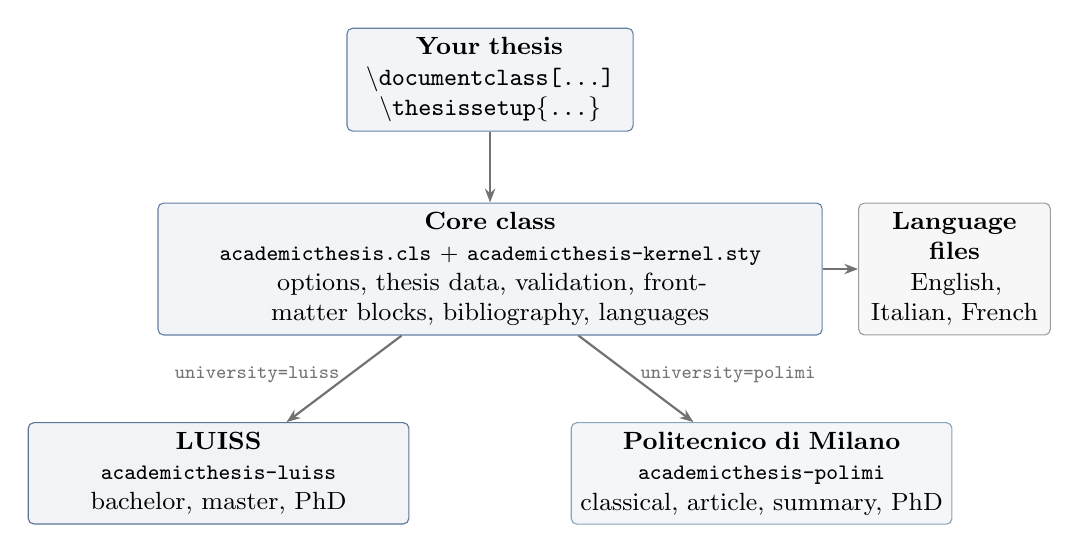
\begin{tikzpicture}[
    box/.style={draw=#1!70, fill=#1!6, rounded corners=2pt, align=center,
                minimum height=1.25cm, text width=3.4cm, font=\small},
    box/.default=docaccent,
    arr/.style={-{Stealth[length=5pt]}, draw=docgrey, thick}]
  \node[box] (user) {\textbf{Your thesis}\\\texttt{\textbackslash documentclass[...]}\\\texttt{\textbackslash thesissetup\{...\}}};
  \node[box, below=0.9cm of user, text width=8.2cm] (core)
    {\textbf{Core class}\\{\footnotesize\texttt{academicthesis.cls} + \texttt{academicthesis-kernel.sty}}\\
     options, thesis data, validation, front-matter blocks, bibliography, languages};
  \node[box=luissblue, text width=4.6cm, below left=1.1cm and -3.2cm of core] (luiss)
    {\textbf{LUISS}\\{\footnotesize\texttt{academicthesis-luiss}}\\bachelor, master, PhD};
  \node[box=bluepoli, text width=4.6cm, below right=1.1cm and -3.2cm of core] (polimi)
    {\textbf{Politecnico di Milano}\\{\footnotesize\texttt{academicthesis-polimi}}\\classical, article, summary, PhD};
  \node[box=docgrey, right=0.45cm of core, text width=2.2cm] (lang)
    {\textbf{Language files}\\English, Italian, French};
  \draw[arr] (user) -- (core);
  \draw[arr] (core) -- node[left, font=\scriptsize, color=docgrey, pos=0.45] {\texttt{university=luiss}} (luiss);
  \draw[arr] (core) -- node[right, font=\scriptsize, color=docgrey, pos=0.45] {\texttt{university=polimi}} (polimi);
  \draw[arr] (core) -- (lang);
\end{tikzpicture}
\end{center}

\begin{description}[leftmargin=0pt, labelindent=0pt, itemsep=4pt]
  \item[The core class] (\file{academicthesis.cls}) knows nothing about any
    particular university. It reads the class options, stores the thesis
    data given with \cs{thesissetup}, checks that nothing required is
    missing, loads fonts, languages and the bibliography, and provides the
    blocks every thesis has: abstract, statement of originality,
    acknowledgements and dedication.
  \item[A university package] (\file{academicthesis-<university>.sty})
    contributes everything that is specific to one institution: the base
    class and page geometry, the cover page for each degree, the data that
    institution requires, and its own wording of the labels (for example
    ``Advisor'' instead of ``Supervisor'').
  \item[Language files] hold every printed word, so labels follow the
    language of the thesis. English, Italian and French are provided, and
    a university can override any single label.
\end{description}

The packages find each other \emph{by name only}, never by folder. Once
installed in a \TeX{} tree, a student can therefore install the core and
just one university package; inside the repository, a small search-path
file lets the examples compile directly. Adding a university means adding
one folder, without touching the core or the other universities.

% ======================================================================
\section{The LUISS package}

\pkg{academicthesis-luiss} produces the LUISS Guido Carli thesis layout for
bachelor's, master's and doctoral theses.

\begin{center}
  \preview[0.3\textwidth]{luiss-master-cover}{Bachelor's / master's cover}\hfill
  \preview[0.3\textwidth]{luiss-secondpage}{Second page}\hfill
  \preview[0.3\textwidth]{luiss-phd-cover}{PhD cover}
\end{center}

\begin{itemize}
  \item \textbf{Cover page.} The LUISS logo, the degree programme
    (``Course of \dots''), an optional major and the chair (``Chair of
    \dots''), the title in LUISS blue, then supervisor(s), co-supervisor(s)
    and candidate in labelled columns, and the academic year at the bottom.
  \item \textbf{PhD cover.} Same structure: the department under the logo,
    ``PhD in \dots'' and the doctoral cycle where a bachelor's or master's
    cover has the course and the chair.
  \item \textbf{Second page.} The examination commission (or a statement
    that the thesis has not been defended) and a copyright block. It is
    printed by default and can be switched off.
  \item \textbf{Adjustable cover.} Logo, title, course, major and
    department lines can each be aligned left, centre or right with
    \cs{luissthesissetup}; the logo size and file can be changed too.
  \item \textbf{Defaults.} \pkg{book} base class; author--year
    bibliography (\pkg{biblatex} with \pkg{biber}).
\end{itemize}

% ======================================================================
\section{The Politecnico di Milano package}

\pkg{academicthesis-polimi} reproduces the thesis layouts of Politecnico di
Milano. One option, \opt{format}, chooses among four of them; the package
then picks the right base class, page size, colours, cover and headings.

\begin{center}
  \preview[0.225\textwidth]{polimi-classical-cover}{\opt{classical}}\hfill
  \preview[0.225\textwidth]{polimi-article-cover}{\opt{article}}\hfill
  \preview[0.225\textwidth]{polimi-summary-cover}{\opt{summary}}\hfill
  \preview[0.18\textwidth]{polimi-phd-cover}{\opt{phd}}
\end{center}

\begin{tabularx}{\textwidth}{@{}l Y l@{}}
\toprule
\textbf{Format} & \textbf{What it is} & \textbf{Built on} \\
\midrule
\opt{classical} & The full thesis as a book: cover page, abstracts, chapters. The default. & \pkg{book}, 12pt, two-sided, A4 \\
\opt{article}   & The thesis as a paper: a header block with the abstract on page~1, then sections. & \pkg{article}, 11pt, A4 \\
\opt{summary}   & The Executive Summary: two columns under a blue page header. & \pkg{article}, 11pt, two columns, A4 \\
\opt{phd}       & The doctoral dissertation. & \pkg{book}, 10pt, 17$\times$24\,cm or A4 \\
\bottomrule
\end{tabularx}

Every PoliMi thesis has an English and an Italian abstract, so both
languages are always loaded. Labels follow PoliMi's own wording
(``Advisor'', ``Student ID'', ``Tesi di Laurea Magistrale in'') in English
or Italian, according to the language of the thesis.

\begin{notebox}[bluepoli]{Credit: the PoliMi layouts are Politecnico di Milano's design}
The page designs reproduced by \pkg{academicthesis-polimi} are \textbf{not
original work of this project}. They come from the official \LaTeX{}
templates provided by Politecnico di Milano:
\begin{itemize}
  \item the thesis templates of the School of Industrial and Information
    Engineering (Scuola di Ingegneria Industriale e dell'Informazione,
    ``Scuola 3I''), revision of October 2021: \emph{Thesis classical
    format}, \emph{Thesis article format} and \emph{Executive Summary},
    on which the \opt{classical}, \opt{article} and \opt{summary} formats
    are modelled;
  \item the PoliMi doctoral dissertation template (\file{phdthesis.sty},
    \file{phdtitle.sty}), on which the \opt{phd} format is modelled.
\end{itemize}
The cover arrangement, colours (\opt{bluepoli}), chapter and section
styles, running headers, the ``raggiera'' background and the Politecnico
logos and seal all belong to Politecnico di Milano and its template
authors. This package re-implements those layouts on top of the shared
\pkg{academicthesis} core, so that they are selected with a class option
and share the core's data handling, validation and multilingual blocks.
The credit for the design goes to Politecnico di Milano.
\end{notebox}

% ======================================================================
\section{What both packages share}

Because both packages sit on the same core, a thesis gets the same
behaviour whichever university it is written for:

\begin{itemize}
  \item \textbf{One place for the data.} Title, candidate, degree,
    supervisors, academic year and the rest are given once, with
    \cs{thesissetup}, using the same key names at every university.
  \item \textbf{Clear errors.} A missing required field stops the
    compilation with a message naming the field and showing an example,
    instead of producing a cover with a blank space.
  \item \textbf{Several languages in one thesis.} The abstract,
    statement of originality, acknowledgements and dedication each take a
    \opt{language} option, so an English thesis can carry an Italian
    abstract with the correct heading, ``Keywords'' label and hyphenation.
  \item \textbf{Counting and gender.} Labels switch between
    ``Supervisor'' and ``Supervisors'' by themselves, and in Italian between
    ``Candidato'' and ``Candidata''.
  \item \textbf{Bibliography that always compiles.} \pkg{biblatex} with
    \pkg{biber} is used when available, with a fallback to \pkg{natbib} and
    Bib\TeX{} behind the same two commands, \cs{addbibresource} and
    \cs{printbibliography}.
  \item \textbf{Nothing imposed beyond the layout.} Each package loads
    only what its layout needs; \pkg{hyperref}, \pkg{tikz}, extra maths
    packages and the bibliography style remain the student's choice.
\end{itemize}

% ======================================================================
\section{Where to go next}

\begin{itemize}
  \item The \textbf{User guide}
    (\file{academicthesis-user-guide.pdf}, in this folder) explains every
    class option and data field, lists what each university and format
    requires, and gives complete examples.
  \item The \textbf{showcases} (\file{showcases/} in the repository) are
    complete theses that compile as they are; copying the one closest to
    your case is the fastest way to start.
  \item The \textbf{architecture guide} (\file{doc/ARCHITECTURE.md}) is
    for those who want to add a university or a language.
\end{itemize}

% ======================================================================
\section*{Acknowledgements and licence}
\addcontentsline{toc}{section}{Acknowledgements and licence}

The \pkg{academicthesis} core class and its packages are released under
the \LaTeX{} Project Public Licence (LPPL) 1.3c or later; copyright
2025--2026 Luca Salvatore.

The Politecnico di Milano layouts are based on the official templates of
Politecnico di Milano, as detailed in the box above; their design, and the
Politecnico di Milano name, logos, seal and graphic elements, belong to
Politecnico di Milano. The LUISS name and logo belong to LUISS Guido Carli.
\pkg{academicthesis} is not published by either university: before
submitting a thesis, always check the current rules of your school or
doctoral programme.

\end{document}
